\documentclass{standalone}
\usepackage{tikz}
\usetikzlibrary{positioning,fit,matrix}
\usepackage{todonotes}
%\usepackage{scalefnt}

%\tikzset{%
%  textnode/.style     = {\sffamily font=\fontsize{10}{12.4}\selectfont},
%}

\begin{document}

\sffamily%\sansmath
%\scalefont{0.01}
%\fontsize{8}{10.0}\selectfont

\begin{tikzpicture}


% L1
\node[inner sep=0] (A) {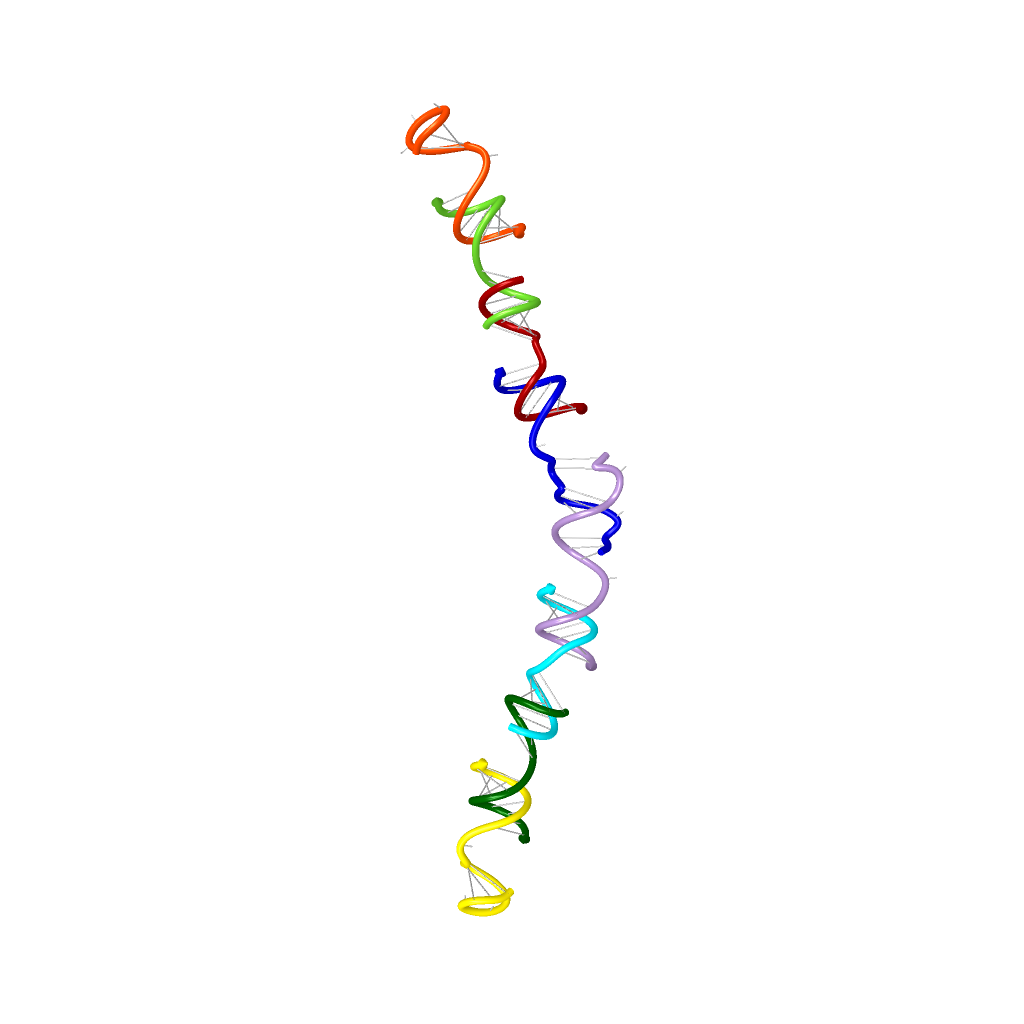
\includegraphics[width=5cm]{3d/L1-A_random.png}};
\node[inner sep=0, below=0mm of A] (B) {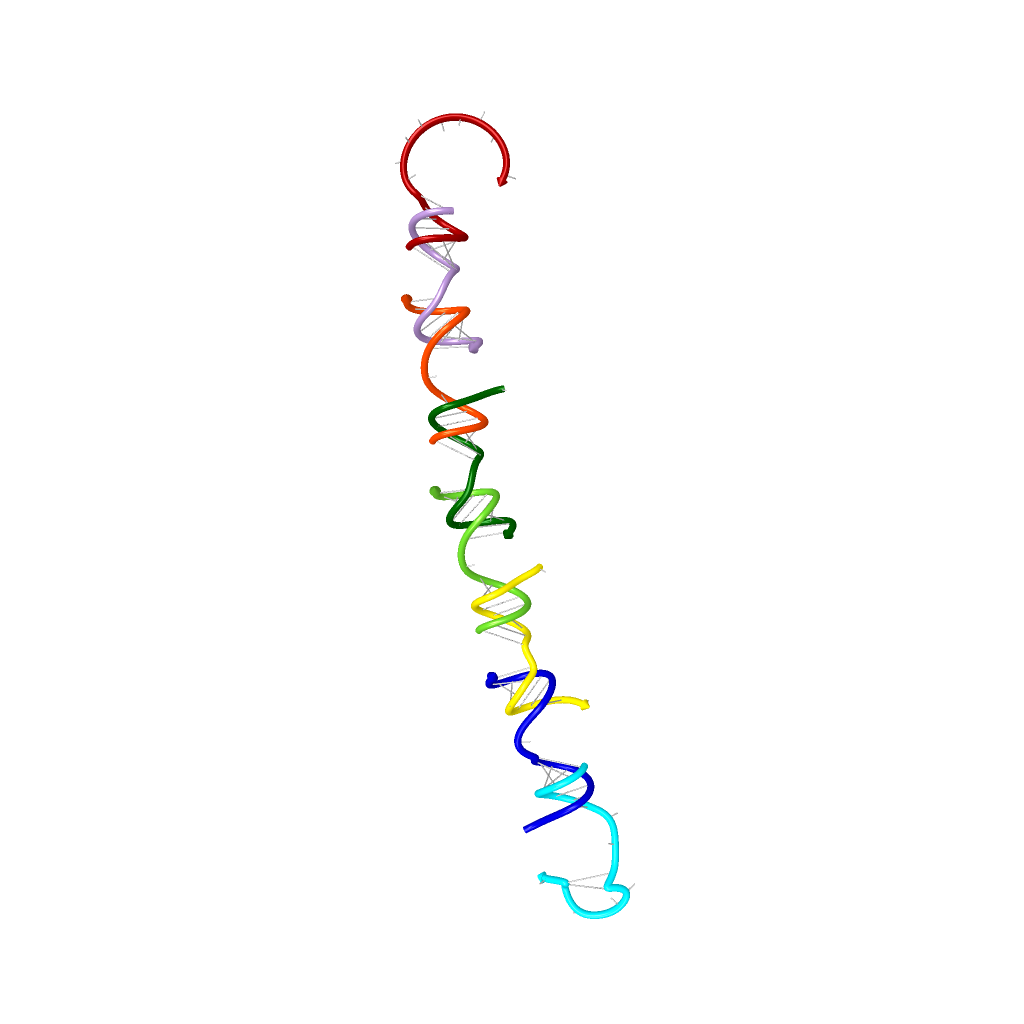
\includegraphics[width=5cm]{3d/L1-B_random.png}};
\node[inner sep=0, below=0mm of B] (C) {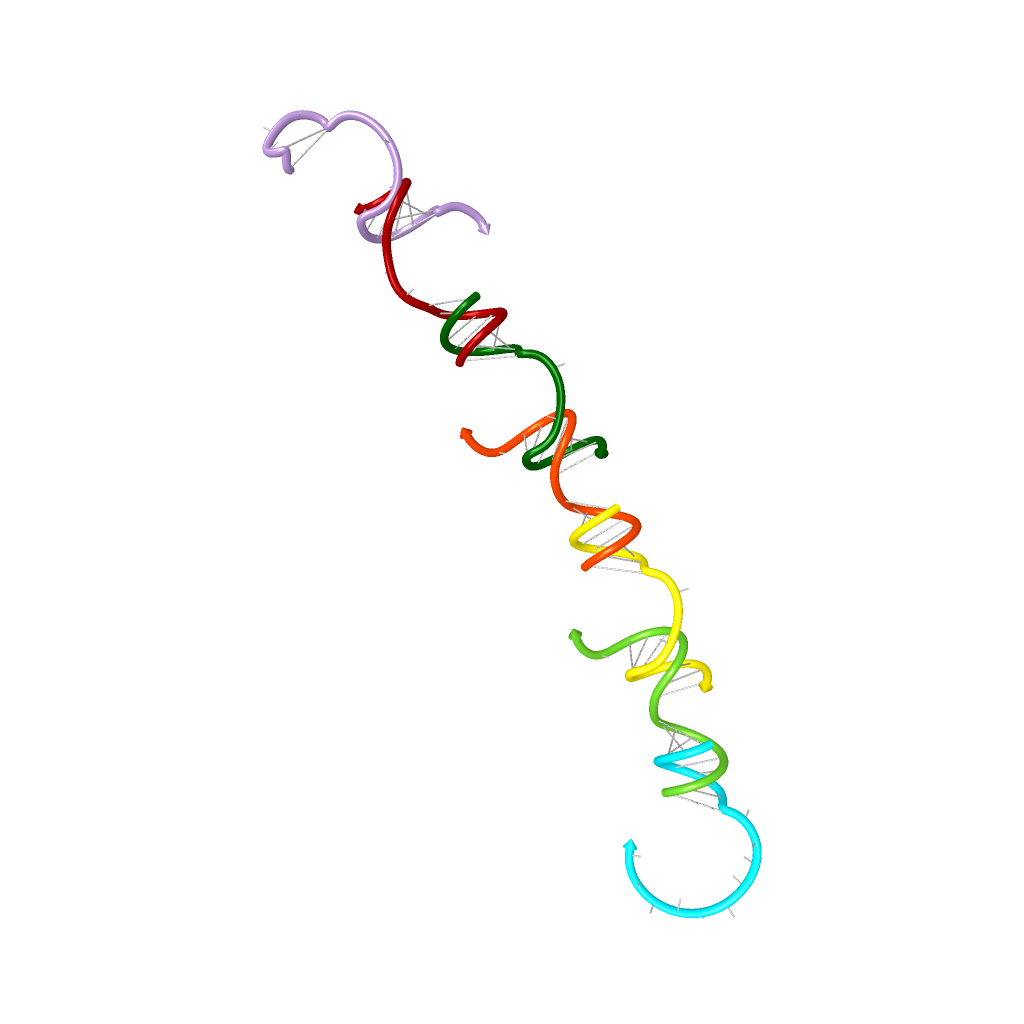
\includegraphics[width=5cm]{3d/L1-C_random.png}};
\node[inner sep=0, below=0mm of C] (D) {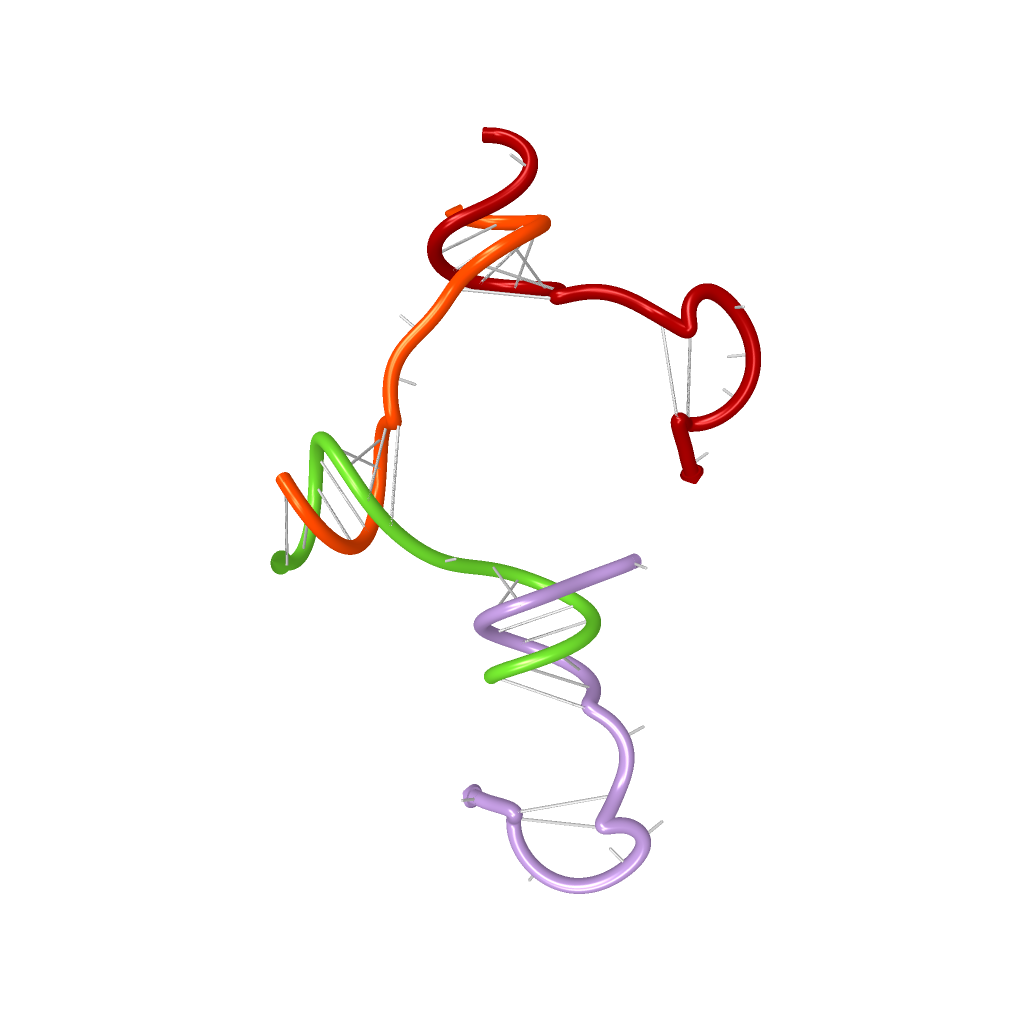
\includegraphics[width=5cm]{3d/L1-D_random.png}};

% L2
\node[inner sep=0, right=5mm of A] (E) {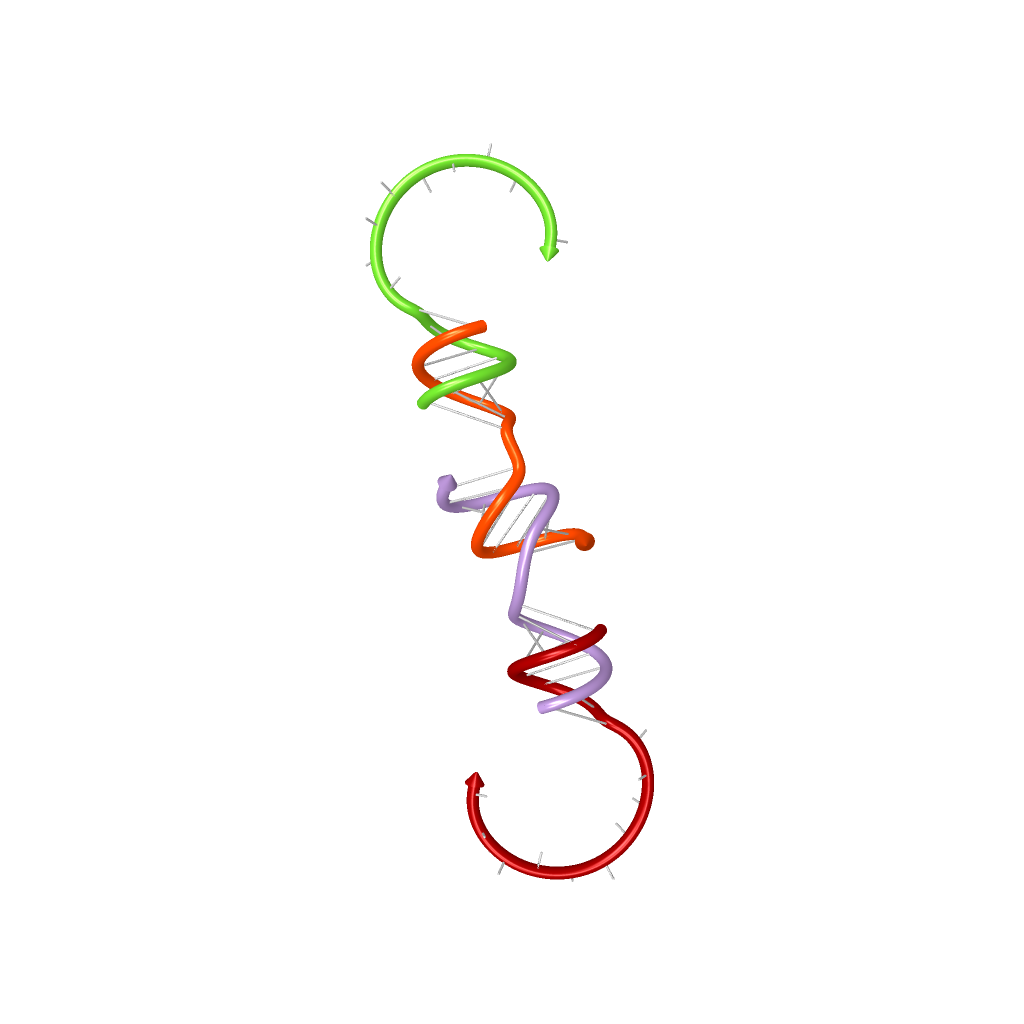
\includegraphics[width=5cm]{3d/L2-E_random.png}};
\node[inner sep=0, below=0mm of E] (F) {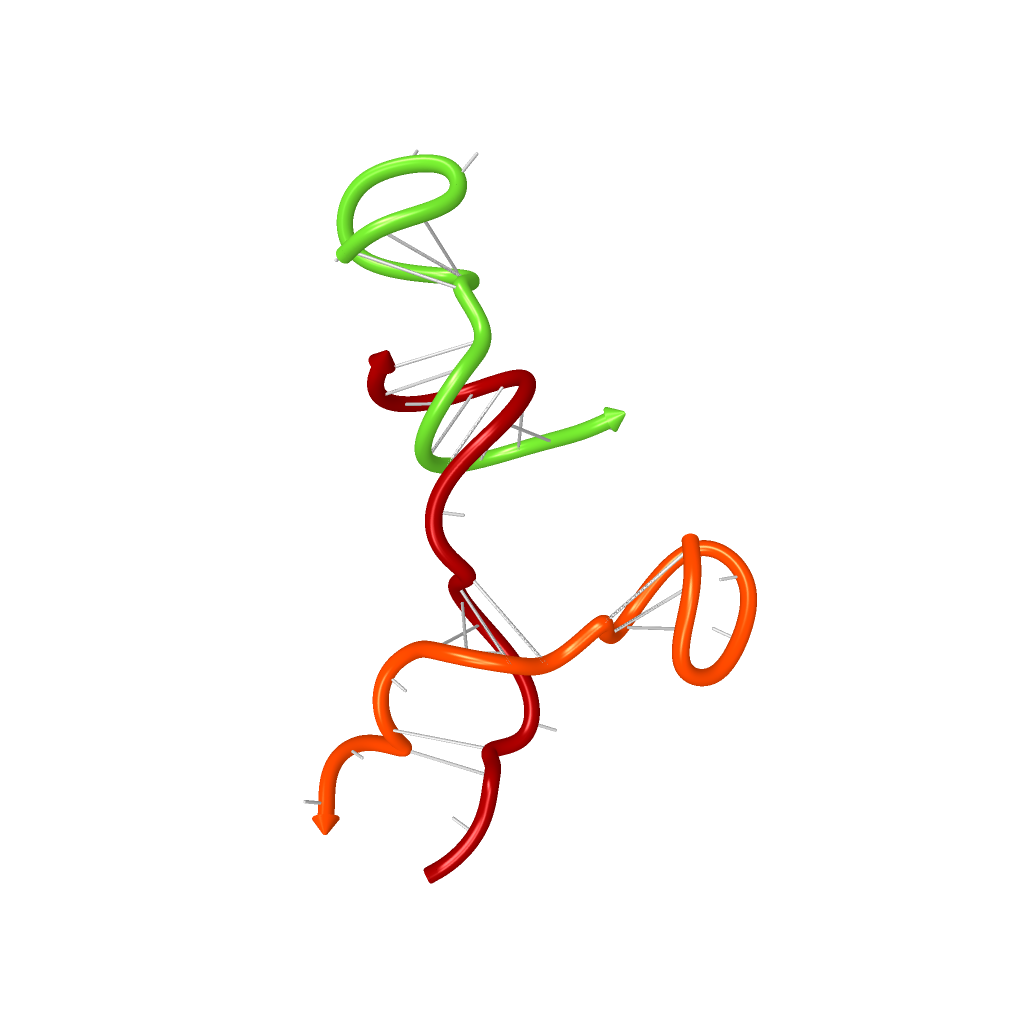
\includegraphics[width=5cm]{3d/L2-F_GA.png}};
\node[inner sep=0, below=0mm of F] (G) {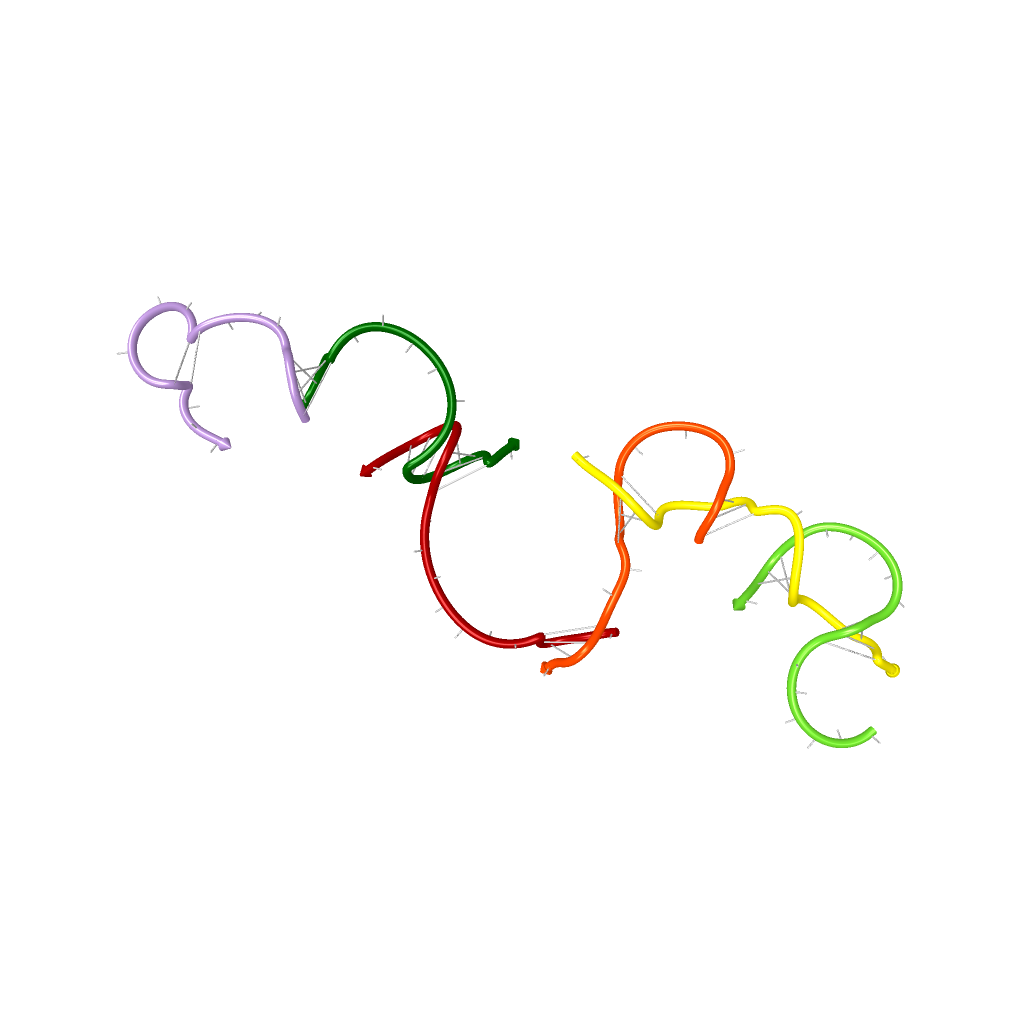
\includegraphics[width=5cm]{3d/L2-G_GA.png}};
\node[inner sep=0, below=0mm of G] (H) {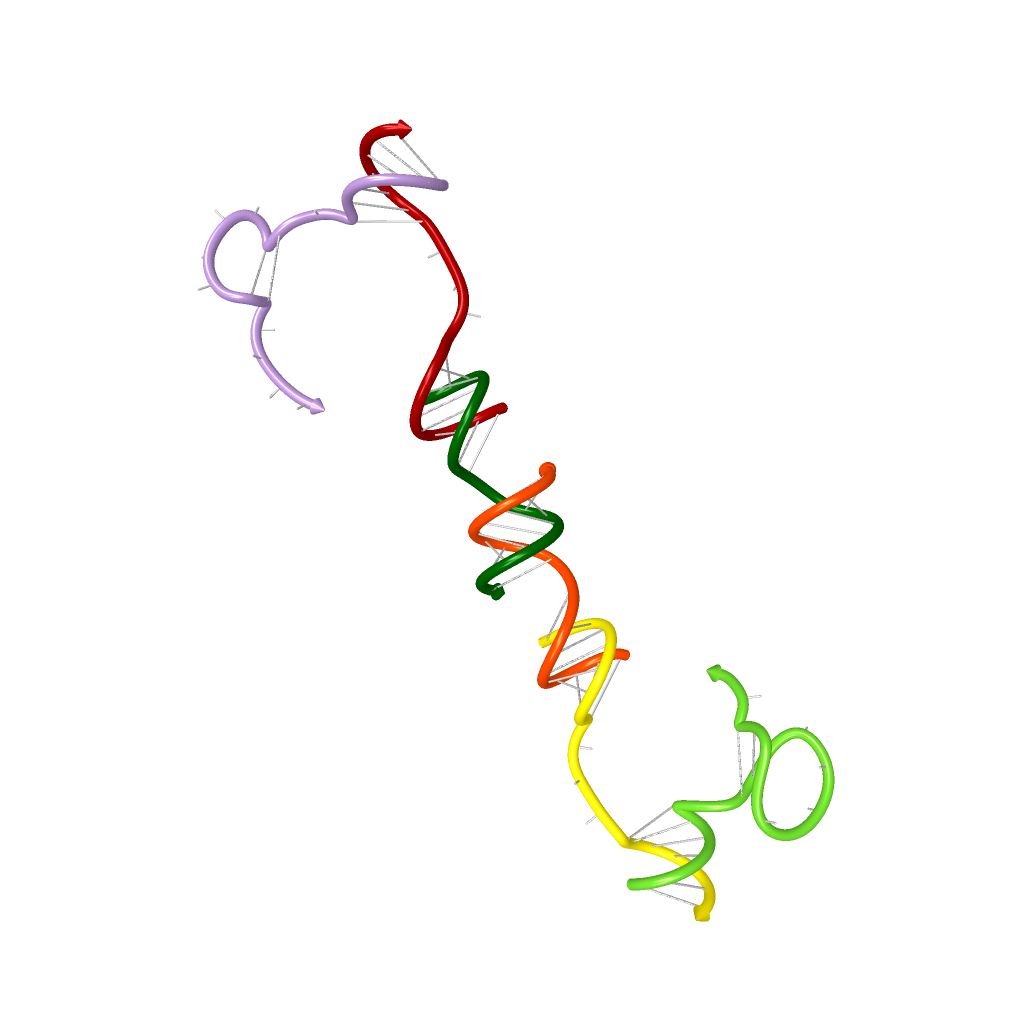
\includegraphics[width=5cm]{3d/L2-H_random.png}};

% L3
\node[inner sep=0, right=5mm of E] (I) {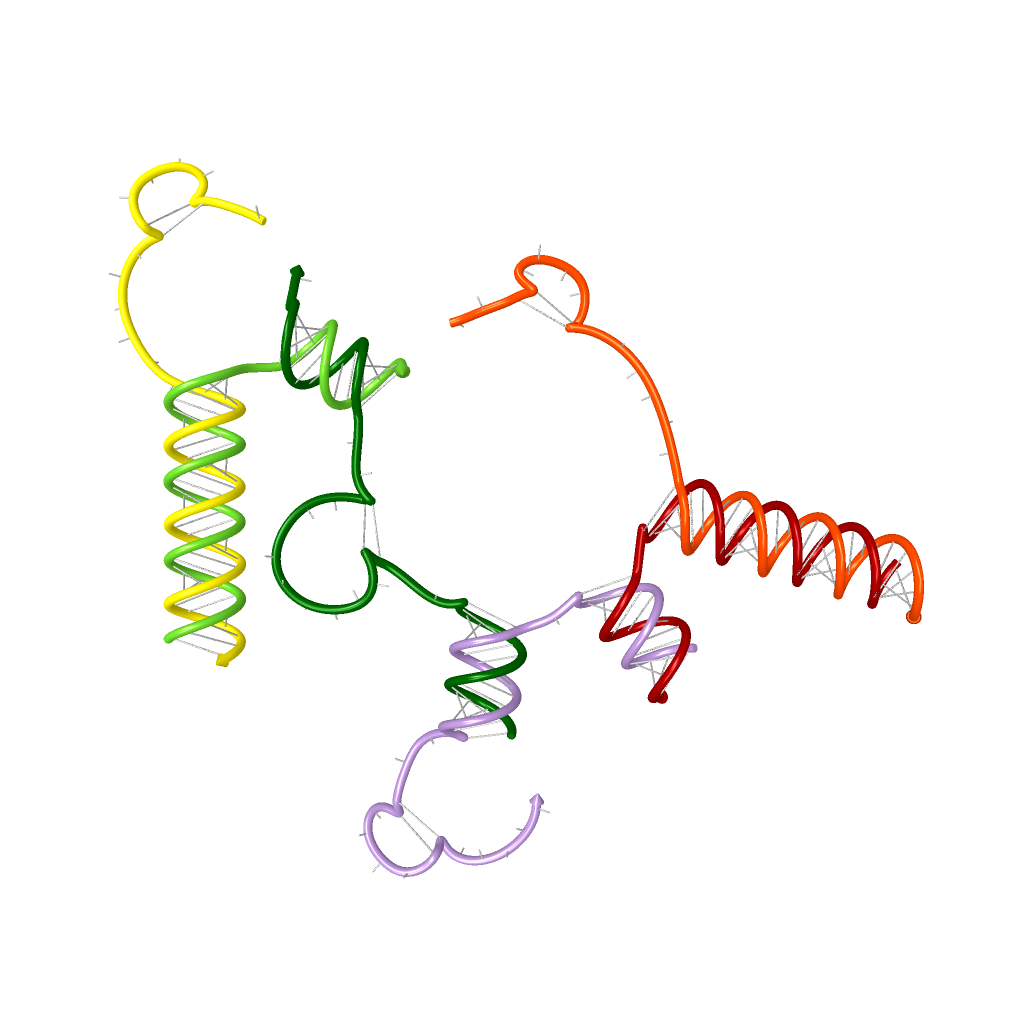
\includegraphics[width=5cm]{3d/L3-I_random.png}};
\node[inner sep=0, below=0mm of I] (J) {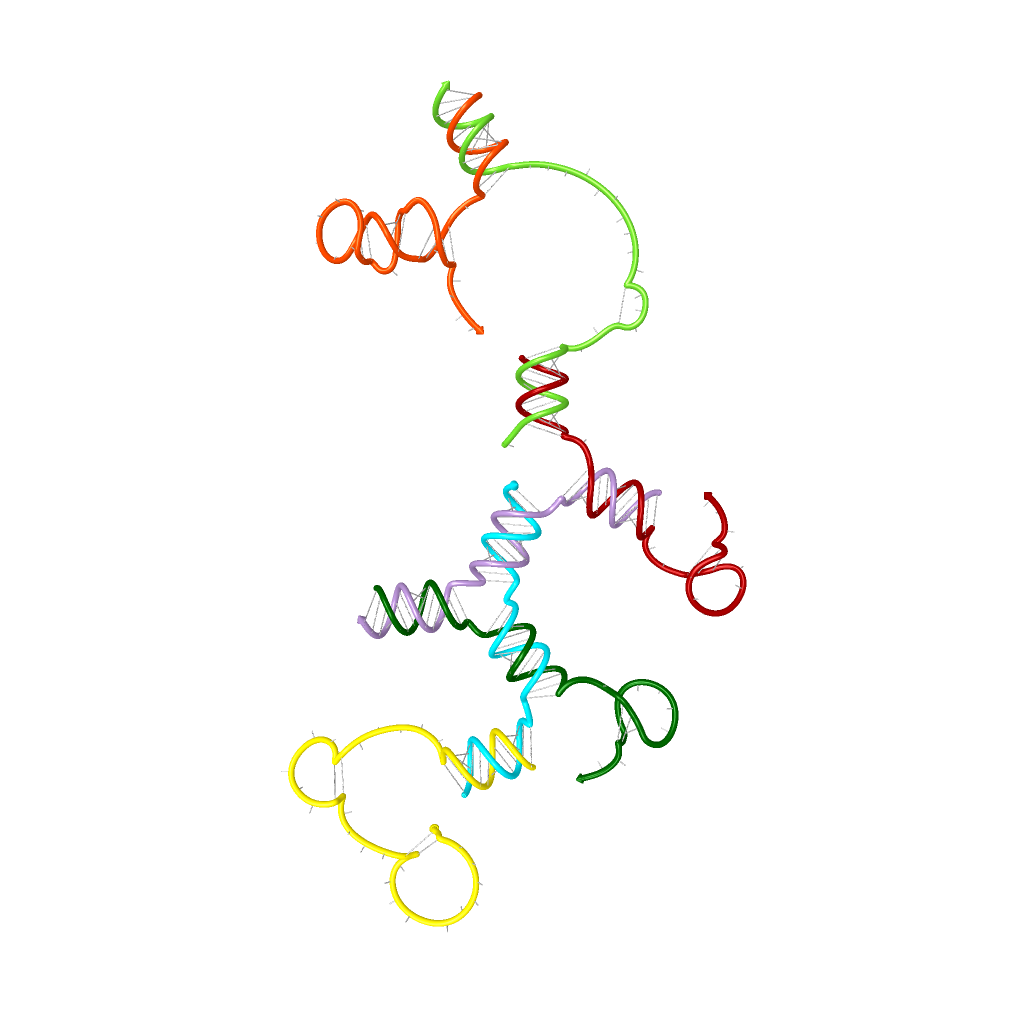
\includegraphics[width=5cm]{3d/L3-J_random.png}};
\node[inner sep=0, below=0mm of J] (K) {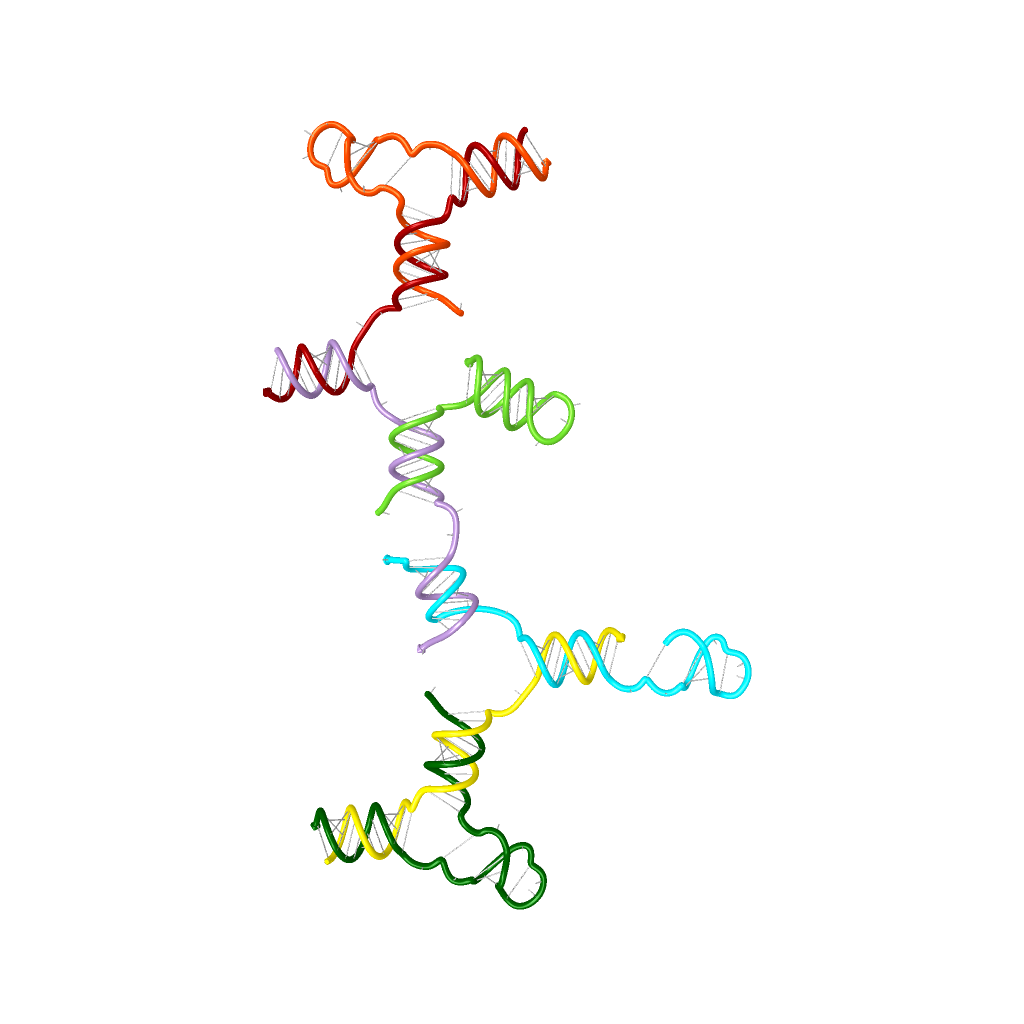
\includegraphics[width=5cm]{3d/L3-K_random.png}};
\node[inner sep=0, below=0mm of K] (L) {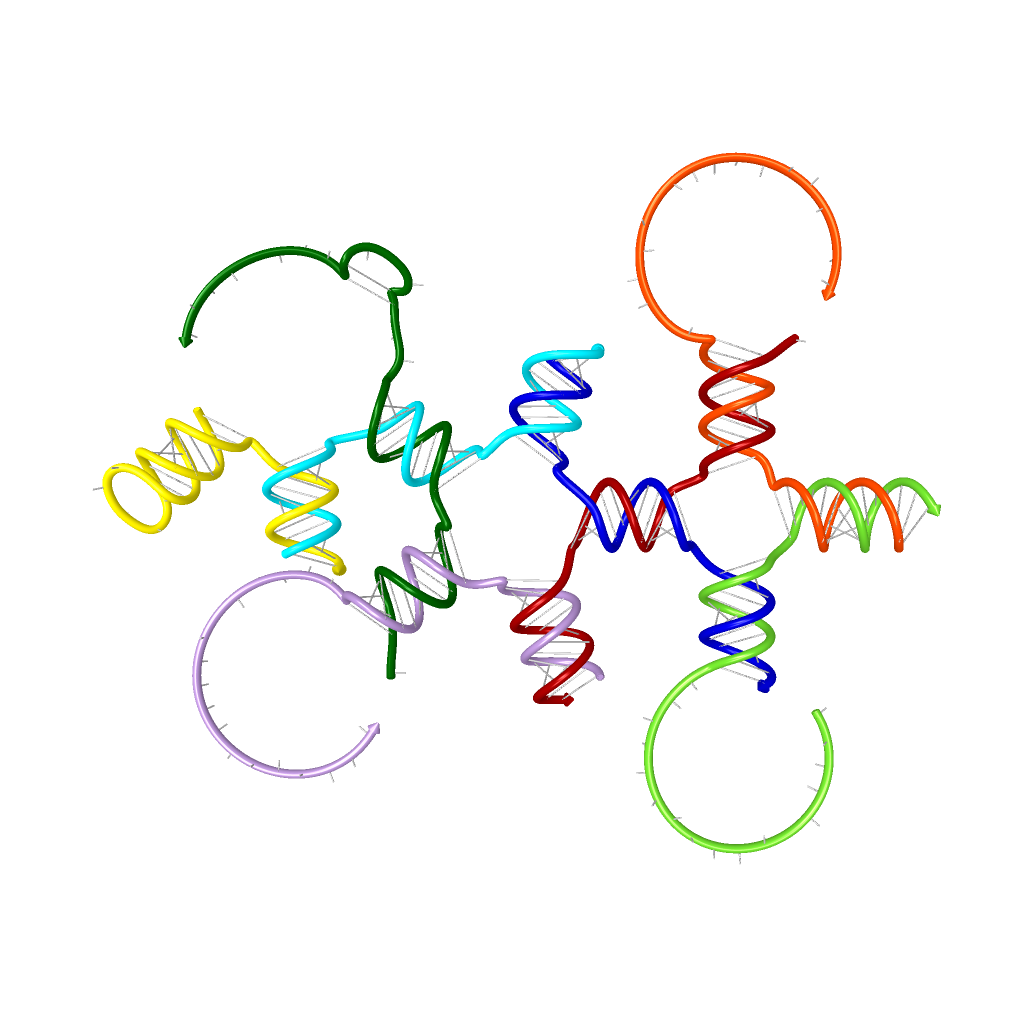
\includegraphics[width=5cm]{3d/L3-L_GA.png}};

% Titles
\node[color=black,above=4mm of A,rotate=0,anchor=north,align=center,shift={(0.00,0.00)}] {\Large{L1}};
\node[color=black,above=4mm of E,rotate=0,anchor=north,align=center,shift={(0.00,0.00)}] {\Large{L2}};
\node[color=black,above=4mm of I,rotate=0,anchor=north,align=center,shift={(0.00,0.00)}] {\Large{L3}};

\node[color=black,left=0.5mm of A,rotate=0,anchor=north,align=center,shift={(1.00,2.40)}] {A};
\node[color=black,left=0.5mm of B,rotate=0,anchor=north,align=center,shift={(1.00,2.40)}] {B};
\node[color=black,left=0.5mm of C,rotate=0,anchor=north,align=center,shift={(1.00,2.40)}] {C};
\node[color=black,left=0.5mm of D,rotate=0,anchor=north,align=center,shift={(1.00,2.40)}] {D};
\node[color=black,left=0.5mm of E,rotate=0,anchor=north,align=center,shift={(1.00,2.40)}] {E};
\node[color=black,left=0.5mm of F,rotate=0,anchor=north,align=center,shift={(1.00,2.40)}] {F};
\node[color=black,left=0.5mm of G,rotate=0,anchor=north,align=center,shift={(1.00,2.40)}] {G};
\node[color=black,left=0.5mm of H,rotate=0,anchor=north,align=center,shift={(1.00,2.40)}] {H};
\node[color=black,left=0.5mm of I,rotate=0,anchor=north,align=center,shift={(1.00,2.40)}] {I};
\node[color=black,left=0.5mm of J,rotate=0,anchor=north,align=center,shift={(1.00,2.40)}] {J};
\node[color=black,left=0.5mm of K,rotate=0,anchor=north,align=center,shift={(1.00,2.40)}] {K};
\node[color=black,left=0.5mm of L,rotate=0,anchor=north,align=center,shift={(1.00,2.40)}] {L};


%% L1
%\node[inner sep=0] (baseline1) {\includegraphics[width=5cm]{plots/peppercorn-L1-meanStruct.pdf}};
%\node[inner sep=0, right=0mm of baseline1] (baseline2) {\includegraphics[width=5cm]{plots/peppercorn-L1-entropyReactionTypes.pdf}};
%%\node[inner sep=0, right=0mm of baseline2] (baseline3) {\includegraphics[width=5cm]{plots/nupack-L1-combined.pdf}};
%
%
%% L2
%\node[inner sep=0, below=0mm of baseline1] (alex1) {\includegraphics[width=5cm]{plots/peppercorn-L2-meanStruct.pdf}};
%\node[inner sep=0, right=0mm of alex1] (alex2) {\includegraphics[width=5cm]{plots/peppercorn-L2-entropyReactionTypes.pdf}};
%%\node[inner sep=0, right=0mm of alex2] (alex3) {\includegraphics[width=5cm]{plots/nupack-L2-combined.pdf}};
%
%
%% L3
%\node[inner sep=0, below=0mm of alex1] (tetra1) {\includegraphics[width=5cm]{plots/peppercorn-L3-meanStruct.pdf}};
%\node[inner sep=0, right=0mm of tetra1] (tetra2) {\includegraphics[width=5cm]{plots/peppercorn-L3-entropyReactionTypes.pdf}};
%%\node[inner sep=0, right=0mm of tetra2] (tetra3) {\includegraphics[width=5cm]{plots/nupack-L3-combined.pdf}};
%
%
%% CBar
%\node[inner sep=0, below=0mm of tetra1] (cbar1) {\includegraphics[width=5cm]{plots/peppercorn-cbar-meanStruct.pdf}};
%\node[inner sep=0, right=0mm of cbar1] (cbar2) {\includegraphics[width=5cm]{plots/peppercorn-cbar-entropyReactionTypes.pdf}};
%%\node[inner sep=0, right=0mm of cbar2] (cbar3) {\includegraphics[width=5cm]{plots/nupack-cbar-combined.pdf}};
%
%
%% Titles
%\node[color=black,above=5mm of baseline1,rotate=0,anchor=north,align=center,shift={(0.20,0.00)}] {Mean Struct. Size};
%\node[color=black,above=5mm of baseline2,rotate=0,anchor=north,align=center,shift={(0.20,0.00)}] {Entropy React. Types};
%%\node[color=black,above=5mm of baseline3,rotate=0,anchor=north,align=center,shift={(0.20,0.00)}] {Nupack Entropy Struct. Size};
%
%\node[color=black,above=1.5mm of baseline1,rotate=0,anchor=north,align=center,shift={(-1.60,0.00)}] {\tiny{$k=(2,3)$}};
%\node[color=black,above=1.5mm of baseline1,rotate=0,anchor=north,align=center,shift={(0.20,0.00)}] {\tiny{$k=(4,5)$}};
%\node[color=black,above=1.5mm of baseline1,rotate=0,anchor=north,align=center,shift={(2.00,0.00)}] {\tiny{$k=(6,7)$}};
%\node[color=black,above=1.5mm of baseline2,rotate=0,anchor=north,align=center,shift={(-1.60,0.00)}] {\tiny{$k=(2,3)$}};
%\node[color=black,above=1.5mm of baseline2,rotate=0,anchor=north,align=center,shift={(0.20,0.00)}] {\tiny{$k=(4,5)$}};
%\node[color=black,above=1.5mm of baseline2,rotate=0,anchor=north,align=center,shift={(2.00,0.00)}] {\tiny{$k=(6,7)$}};
%%\node[color=black,above=1.5mm of baseline3,rotate=0,anchor=north,align=center,shift={(-1.60,0.00)}] {\tiny{$k=(2,3)$}};
%%\node[color=black,above=1.5mm of baseline3,rotate=0,anchor=north,align=center,shift={(0.20,0.00)}] {\tiny{$k=(4,5)$}};
%%\node[color=black,above=1.5mm of baseline3,rotate=0,anchor=north,align=center,shift={(2.00,0.00)}] {\tiny{$k=(6,7)$}};
%
%\node[color=black,left=3mm of baseline1,rotate=90,anchor=north,align=center,shift={(0.0,0.0)}] {\textbf{L1}};
%\node[color=black,left=3mm of alex1,rotate=90,anchor=north,align=center,shift={(0.0,0.0)}] {\textbf{L2}};
%\node[color=black,left=3mm of tetra1,rotate=90,anchor=north,align=center,shift={(0.0,0.0)}] {\textbf{L3}};
%


\end{tikzpicture}

\end{document}
